\documentclass[a4paper,12pt]{article}

\usepackage[margin=2.5cm]{geometry}
%\usepackage{mathpazo}
\usepackage{amsmath,amssymb}
\usepackage{graphicx}
\usepackage[usenames,dvipsnames]{color}
\usepackage{float}
\usepackage{colortbl}
\usepackage{amsthm}
\usepackage{units}
\usepackage{mathabx}
\usepackage{hyperref}
\usepackage{xspace}
\usepackage[noend]{algorithmic}
\renewcommand{\to}{\textbf{ to }}
\changenotsign

\definecolor{DarkBlue}{rgb}{0.00,0.00,0.55}
\hypersetup{
    linkcolor   = DarkBlue,
    anchorcolor = DarkBlue,
    citecolor   = DarkBlue,
    filecolor   = DarkBlue,
    pagecolor   = DarkBlue,
    urlcolor    = DarkBlue,
    colorlinks  = true,
    pdftitle    = {Numerical Methods 1},
}


\definecolor{paleblue}{rgb}{0.9,0.95,1.0}
\definecolor{palegrey}{rgb}{0.9,0.9,0.9}

%\renewcommand{\chaptername}{Lecture}


\usepackage[T1]{fontenc}
\usepackage[sc]{mathpazo}
%\linespread{1.05}

%\newcommand{\lecture}[1]{\chapter{#1}}

\newcommand{\real}[1]{\mathrm{Re}(#1)}
\newcommand{\imag}[1]{\mathrm{Im}(#1)}
\renewcommand{\d}{\mathrm{d}}
\newcommand{\dx}{\,\d x}
\newcommand{\dy}{\,\d y}
\newcommand{\dt}{\,\d t}
\newcommand{\ddx}[2][x]{\frac{\d#2}{\d#1}}
\newcommand{\ddxx}[2][x]{\frac{\d^2#2}{\d#1^2}}
\newcommand{\ddt}[2][t]{\frac{\d#2}{\d#1}}
\newcommand{\ddtt}[2][t]{\frac{\d^2#2}{\d#1^2}}
\newcommand{\ppx}[2][x]{\frac{\partial#2}{\partial#1}}
\newcommand{\ppy}[2][y]{\frac{\partial#2}{\partial#1}}
\newcommand{\ppz}[2][z]{\frac{\partial#2}{\partial#1}}
\newcommand{\ppt}[2][\theta]{\frac{\partial#2}{\partial#1}}
\newcommand{\ppr}[2][r]{\frac{\partial#2}{\partial#1}}
\newcommand{\ppxx}[2][x]{\frac{\partial^2#2}{\partial#1^2}}
\newcommand{\mat}[1]{\mathrm{#1}}
\DeclareMathOperator{\len}{len}

\newcommand{\A}{\mat A}
\newcommand{\AT}{\mat A^{\mat T}}
\renewcommand{\L}{\mat L}
\newcommand{\U}{\mat U}
\renewcommand{\P}{\mat P}

\newcommand{\Integer}{\mathbb{Z}}
\newcommand{\Real}{\mathbb{R}}
\newcommand{\Rational}{\mathbb{Q}}
\newcommand{\Complex}{\mathbb{C}}
\newcommand{\Natural}{\mathbb{N}}

\renewcommand{\O}{\ensuremath{\mathcal{O}}\xspace}
\renewcommand{\vec}[1]{\mathbf{#1}}
\newcommand{\x}{\vec{x}}

\newcommand{\fhat}{\hat{f}}

\newcommand{\eps}{\epsilon_{\mathrm{machine}}}

\DeclareMathOperator{\shape}{shape}

\newcommand{\intpi}{\int_{-\pi}^{\pi}}

\theoremstyle{definition}
\newtheorem{exercise}{Exercise}[section]
\newtheorem{theorem}{Theorem}[section]
\newtheorem{corollary}[theorem]{Corollary}
\newtheorem{define}[theorem]{Definition}

\newcommand{\T}{{\color{green}T}}
\newcommand{\F}{{\color{red}F}}

\setlength{\parskip}{2ex}
\setlength{\parindent}{0ex}

\floatstyle{boxed}
\newfloat{biography}{tp}{lob}

\usepackage{listings}

\lstloadlanguages{Python}

\lstset{basicstyle=\ttfamily,framerule=0.5ex, backgroundcolor=\color{paleblue},gobble=2}

\lstnewenvironment{pythonprogram}{\lstset{language=Python,frame=l,rulecolor=\color{blue}}}{}
\lstnewenvironment{pythonsnippet}{\lstset{language=Python}}{}

\lstnewenvironment{bash}{\lstset{language=bash,backgroundcolor=\color{palegrey}}}{}

\lstMakeShortInline[language=Python]{~}

\newcommand{\note}[1]{{\Large\color{red}#1}}

\begin{document}

\title{Introduction to computational science}

\author{Dr David Ham}

\renewcommand{\today}{5 November 2014}

\maketitle

\section{The theory of computational science}

\tableofcontents



\subsection{What is computational science?}

In essence computational science is what you are doing whenever there is a
computation in the chain between your hypothesis and conclusion. This is
true for a huge proportion of modern science - it is exceptionally likely to
be true for at least some of the science you do.

We can broadly split computational science into two arms: simulation and
data processing. Any particular scientific experiment might involve either
or both of these. Figure \ref{fig:science}\ is a cartoon of a scientific
workflow which shows the three main ways of testing a scientific hypothesis:
experiment, observations and simulation. Observe that all of these produce
data and, in modern science, the processing of that data is usually
performed with a computer.

\begin{figure}[ht]
  \centering
  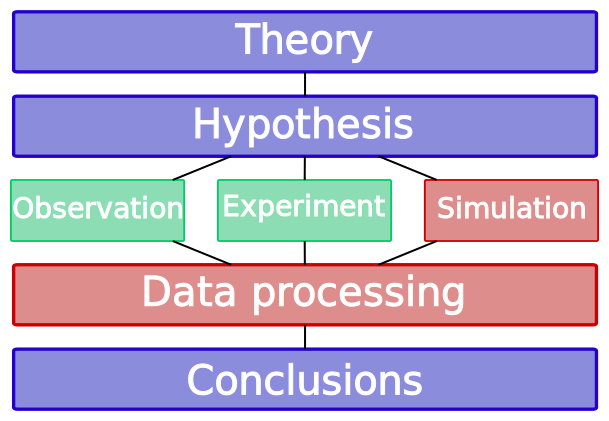
\includegraphics[width=.8\textwidth]{figures/science.pdf}
  \caption{A simplified scientific workflow. The blue boxes are intellectual activities, the green boxes physical and the red boxes computational.}
  \label{fig:science}
\end{figure}

\subsection{The ``lab technique'' of computational science}

A key feature of science is that it should be reproducible: running the
same experiment again should (in some statistical sense) produce the same
results. This critically depends on knowing what you did when you conducted
the experiment.

If you work in an experimental or observational field, you will (hopefully!)
already be familiar with the discipline of laboratory or fieldwork
technique. Whether it is the correct way to hold apparatus, or procedures
for calibrating equipment, disciplines have adopted working practices which
standardise the way scientific work is conducted. These have multiple
functions: they may prevent contamination of results, for example, but a
critical feature of these standardised techniques is that they enable both
the original researcher and users of the science (especially users trying to
reproduce the science) to know what happened. If a subsequent investigation
does not reproduce the original results, good practice also aids the
forensic process of trying to establish why the two experiments produced
different results.

The experimental and observational sciences are on the whole exceptionally
good at this rigorous technique, and they are typically good at educating
students at undegraduate and graduate level in doing this
correctly. Unfortunately, the same cannot be said for computational
techniques. Frequently it is just assumed that the computational science
aspect of a project will just happen and the students will miraculously be
able to do it and will get it right.

Unfortunately when you do a simulation or process data, there are a lot of
things which can go wrong. For example:
\begin{enumerate}
\item There can be derivation mistakes in the calculation you are performing.
\item There can be bugs in your code.
\item You can make human errors processing the data.
\item The approximation errors in the calculations you do may affect the
  accuracy of the solution.
\end{enumerate}
The objective of this lecture is to understand something of the nature of
these challenges, and to give some indication of the tools and procedures
which can protect you from them.

\subsection{Provenance of data and results}

Figure \ref{fig:science} is, of course, a gross simplification of how real
life science problems are solved. A simulation may itself be driven by the
processed data of an experiment or observational campaign, data may be taken
from an experiment and processed to provide feedback, and many different
sorts of data processing may be chained together. This creates a significant
problem for scientists: the user of a scientific result needs to have some
confidence that all of those steps in the chain were actually done
right. This problem creates the issue of provenance: in order to produce a
reliable scientific result it is necessary to be able to trace back the data
which led to that result and establish that every stage of its collection
and processing was correctly undertaken. This creates issues that go beyond
computational science, but the computational science aspects of this are
considerable.
\begin{enumerate}
\item How can one know where data comes from and what processing has
  occurred?
\item Which version of the processing software or script was used?
\item Was that software correct?
\item What was the input data and where does it come from?
\end{enumerate}

\subsection{The paper revision nightmare}

Lest you feel at this point that this sounds rather like a lot of work for a
nebulous philosophical gain, let's examine a situation which is all too
common. You do a tonne of work, and submit a paper to a journal based on
your careful simulations or data analysis. Several months later, the reviews
come back and a reviewer suggests that you need to report some additional
quantity derived from your data. You do the analysis and get an answer which
seems surprising 

\subsection{Two different sorts of truth.}

Before we get into the question of how to go about employing tools and
working practices to overcome these problems.


\subsection{Verification and validation}





\section{The tools of computational science}

\subsection{Scripting}

\subsection{Revision control}

\subsection{Integration testing}

\subsection{Workflow tools?}




\end{document}
